\section{Estudo do comportamento de buscas}
As buscas por palavras-chave estão diretamente ligadas aos anseios dos públicos que queremos atingir. Iniciaremos verificando as tendências de buscas que levam para o site institucional da Procempa atualmente. Conforme a Figura \ref{fig:busca-site} o termo que mais leva ao site é o PortoWeb, serviço desativado e serviços relacionados à Prefeitura, como webmail e trânsito.

\begin{figure}[!h]
  \centering
    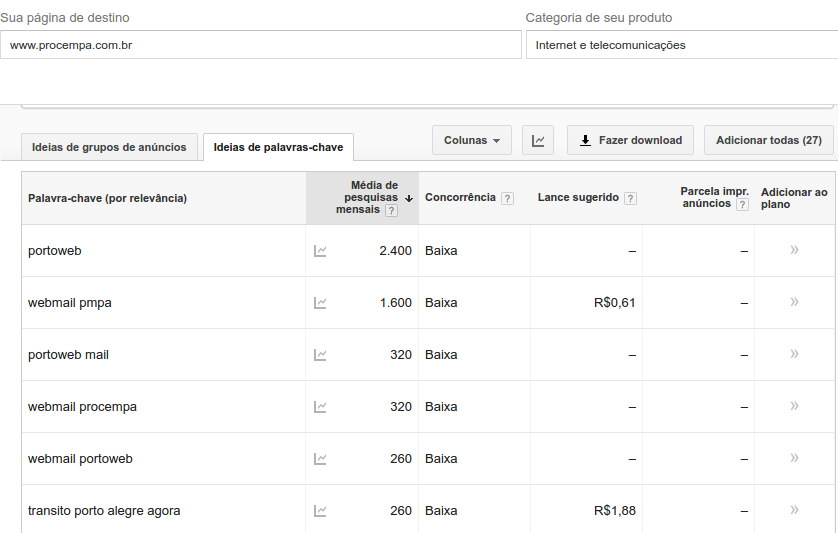
\includegraphics[width=.8\textwidth]{busca-site-procempa}
  \caption{Tendências de Busca Site Procempa}
  \label{fig:busca-site}
\end{figure}

Para atrair novos públicos para o site devemos estabelecer novas palavras para nortearem os conteúdos para o público que queremos atingir. Os formadores de opinião devem buscar por boas práticas na gestão pública, assim produziremos artigos para publicizar as ações de gestão ágil de projetos que temos implementado na companhia. Assim, conforme a Figura \ref{fig:gestao-publica}, deveremos promover conteúdos contendo a palavra chave "Gestão Pública" e seus derivados para melhor ranquearmos nas pesquisas.

\begin{figure}[!h]
  \centering
    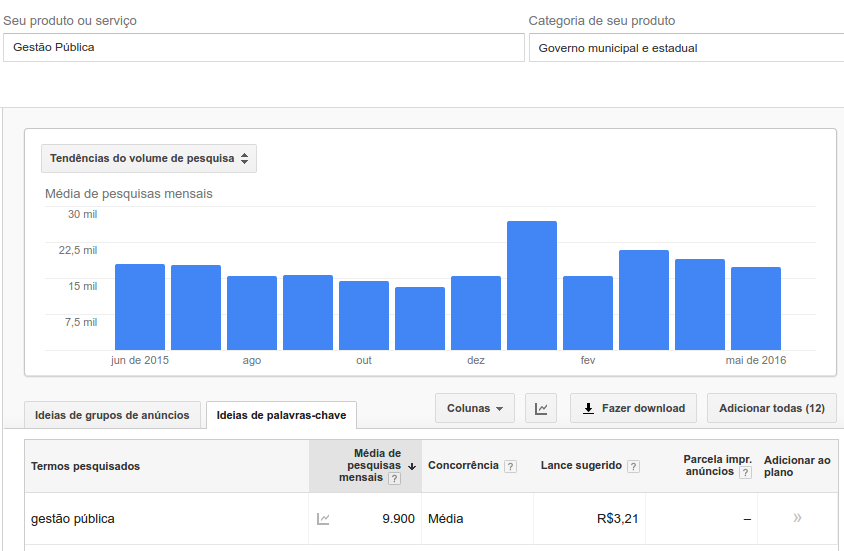
\includegraphics[width=.8\textwidth]{gestao-publica}
  \caption{Palavra Chave Gestão Pública}
  \label{fig:gestao-publica}
\end{figure}

Comunidades de software livre buscarão por iniciativas de código aberto para utilizar em seus próprios projetos. Assim temos que focar em geração de conteúdo útil através do site \citeonline{github} e suas ferramentas como compartilhamento de código e participação em projetos que são parte do dia a dia dos colaboradores. Como vemos na Figura \ref{fig:github-procempa}, atualmente a Companhia possui somente um repositório, já com 8 estrelas mesmo sem nenhum foco de divulgação.

\begin{figure}[!h]
  \centering
    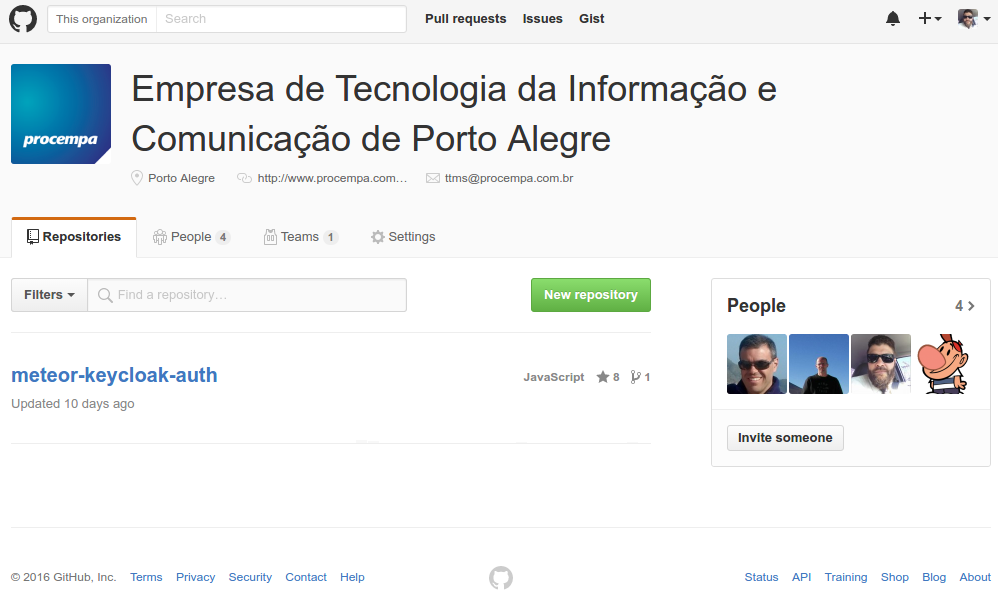
\includegraphics[width=.8\textwidth]{github-procempa}
  \caption{Repositório de Código Procempa no GitHub}
  \label{fig:github-procempa}
\end{figure}

O cidadão da cidade busca por serviços e informações sobre a transparência no trato da coisa pública. Para este público focaremos na parte dos serviços ao cidadão. Como um dos principais serviços com impacto e atendimento direto ao morador ou visitante da cidade, os acessos gratuitos à internet através do \citeonline{poa-livre}, para melhor divulgar esta estratégia o foco será na palavra "Wifi Grátis", conforme as projeções da Figura \ref{fig:wifi-gratis}.

\begin{figure}[!h]
  \centering
    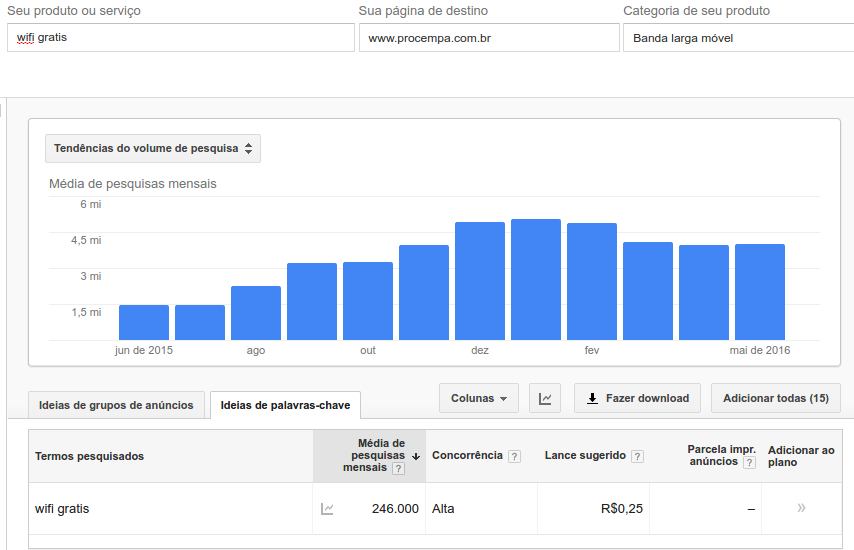
\includegraphics[width=.8\textwidth]{wifi-gratis}
  \caption{Tendências da Palavra Chave Wifi Grátis}
  \label{fig:wifi-gratis}
\end{figure}
